\chapter{METHODOLOGY}    

\section{NHWDTM System Workflow Diagram}
      \begin{figure}[H]
        \centering
        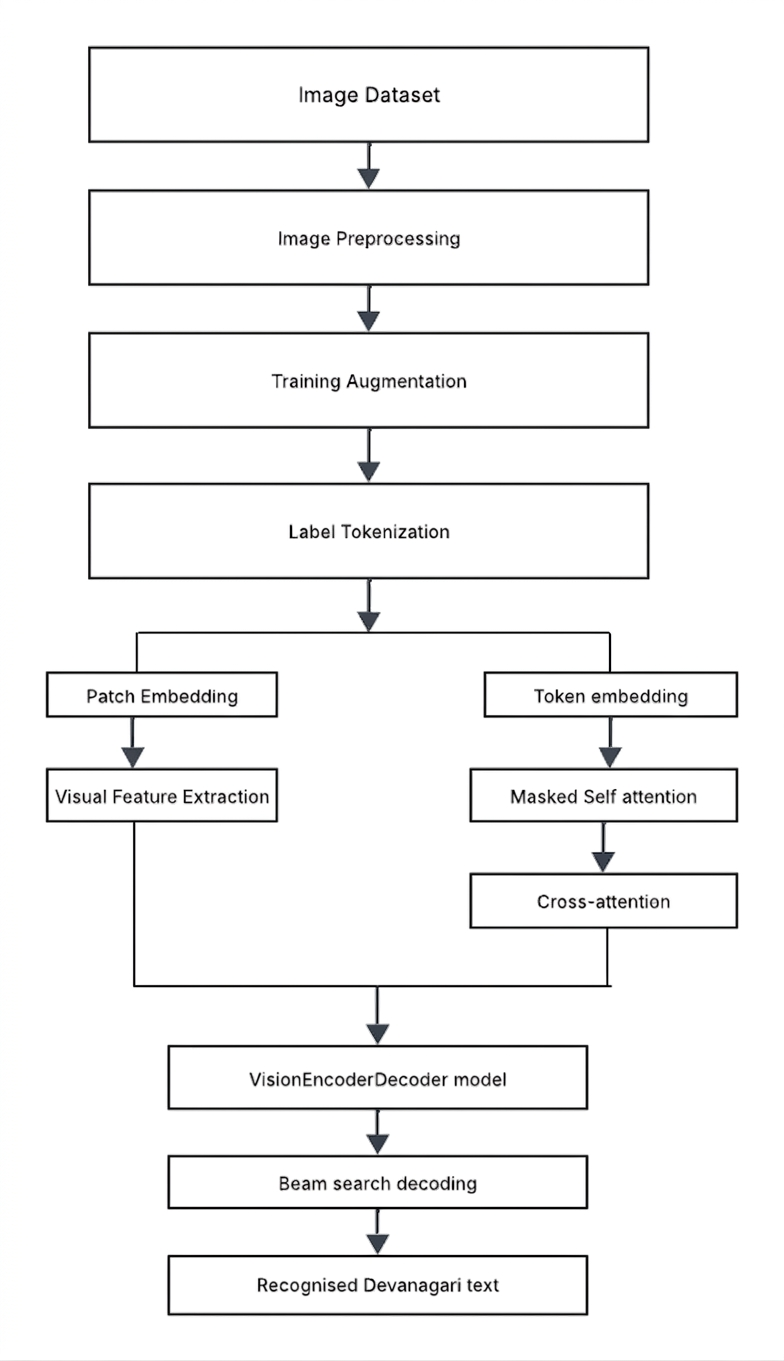
\includegraphics[scale=0.35]{img/system.png}
        \caption{Stages of NHWDTM System}
        \label{fig:blockdiagram}
    \end{figure}

\section{Description of Working Flow of the System}
    \begin{enumerate}
  \subsection{Data Collection:}
Initially, the project was focused on character-level recognition for which,a Devanagari Character Dataset \cite{anand2023devanagari} was used.And,since matras (diacritics) were not well represented, an additional matra dataset was manually created and curated. However, due to lower accuracy and limitations at the character level, the approach was later shifted to word-level recognition using the IIIT-HW-Dev dataset\cite{rajak_indic_data}\Appendices~\ref{app:A.1}.It contains segmented word-level images along with their corresponding Unicode labels. The dataset was obtained from Kaggle and divided into the following splits:
\begin{itemize}
    \item \textbf{Training set:} 69,802 images
    \item \textbf{Validation set:} 12,713 images
    \item \textbf{Test set:} 12,865 images
\end{itemize}
\noindent Each dataset entry includes an image file and its corresponding Unicode label. In total, 108 unique Devanagari characters were identified, including consonants, matras, and compound characters. The maximum label length observed was 23 characters. This dataset provides a diverse and realistic base for training the handwritten word recognition model.
\newpage
  \subsection{Image Pre-processing Pipeline:}\\
   Each image is passed through a multi-step pre-processing pipeline before being fed to the model. The steps are applied in the following order:
  \begin{figure}[H]
        \centering
        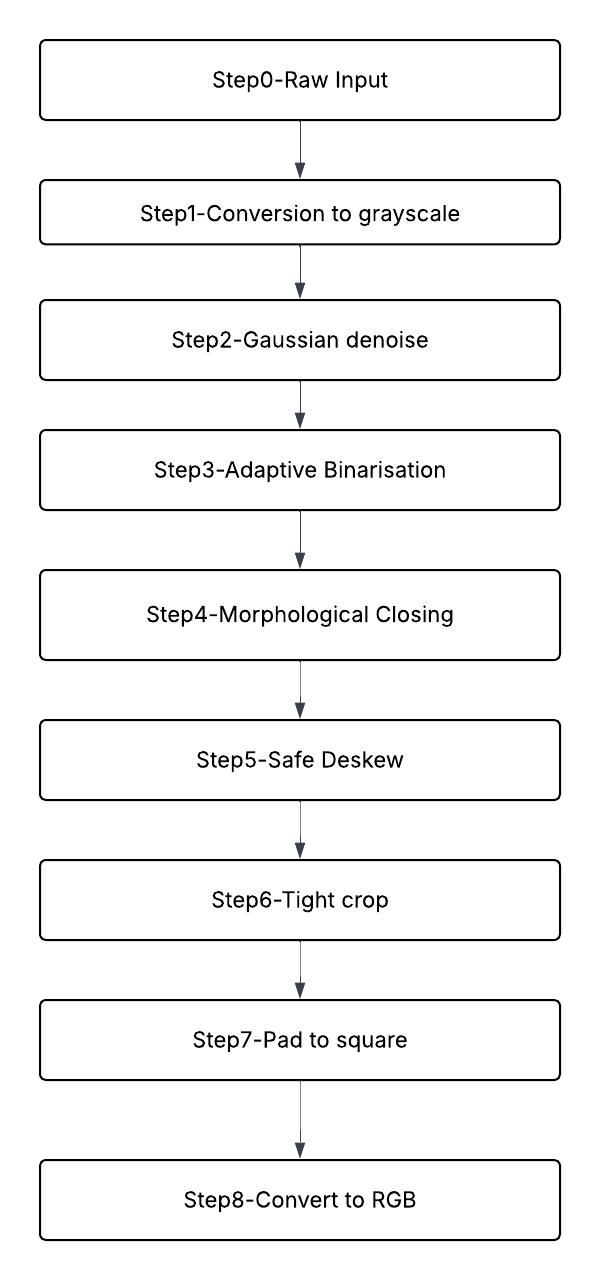
\includegraphics[scale=0.75]{img/Processing.png}
        \caption{Image Pre-processing pipeline}
        \label{fig:processingdiagram}
    \end{figure}
      \begin{itemize}
      \item \textbf{Grayscale conversion and denoising:} The image is converted to grayscale and smoothed with a $3 \times 3$ Gaussian blur to suppress noise while preserving stroke edges.
      \item \textbf{Adaptive binarisation:} An adaptive Gaussian threshold (block size 25, constant $C = 15$) converts the smoothed image to a binary foreground-background representation. This handles uneven
      backgrounds more robustly than global Otsu thresholding.
      \newpage
   \item \textbf{Morphological closing:} A $2 \times 2$ rectangular kernel is used to close small gaps in Devanagari stroke connections, particularly the shirorekha(headline stroke).
      \item \textbf{Deskewing:} Skew angle is estimated using the minimum area bounding rectangle of foreground pixels. Corrections are applied only for angles in the range $[0.5°, 10°]$; larger rotations are ignored to avoid misidentifying vertical strokes as tilt.
      \item \textbf{Tight cropping:} The image is cropped to the bounding box of ink pixels with 8 pixels of padding on each side. Crops smaller than $10 \times 10$ pixels revert to the uncropped image.
      \item \textbf{Letterbox padding and resize:} The cropped image is centred on a white square canvas, then resized to $128 \times 128$ pixels using area interpolation to preserve structural detail.
      \item \textbf{Conversion to RGB and ViT normalisation:} The
      grayscale image is converted to three-channel RGB and passed to
      ViTImageProcessor, which rescales it to $384 \times 384$
      pixels and normalises pixel values to the ViT pre-training
      distribution (mean~$= 0.5$, std~$= 0.5$ per channel).
  \end{itemize}
  All pre-processed images are cached to disk before training to avoid
  repeated computation.
  Detailed before/after visuals for each step are provided in 
Appendices~\ref{app:B1}--\ref{app:B7}
.

  \subsection{Training Data Augmentation:}\\
  During training only, an additional augmentation pipeline is applied on-the-fly after loading the pre-processed image from cache. The augmentations simulate realistic handwriting variation:
  \begin{itemize}
      \item Gaussian blur ($p = 0.4$, $\sigma \in [0.1, 1.0]$)
      \item Random affine transform: rotation $\pm 7°$, translation
      $\pm 7\%$, scale $[0.85, 1.15]$, shear $\pm 5°$
      \item Colour jitter: brightness $\pm 0.4$, contrast $\pm 0.4$,
      saturation $\pm 0.1$
      \item Random perspective distortion ($p = 0.3$,
      distortion scale $= 0.15$)
      \item Random autocontrast ($p = 0.2$)
      \item Random erasing ($p = 0.3$, erased area $2\%$--$12\%$ of
      image)
  \end{itemize}
  Validation and test images are \emph{not} augmented.
\newpage
  \subsection{Custom Tokenizer Construction:}\\
  A character-level tokenizer is built to handle the Devanagari script
  vocabulary. Key properties are:
  \begin{itemize}
      \item \textbf{Vocabulary:} 112 tokens in total ; four special tokens
      (\texttt{<pad>}, \texttt{<s>}, \texttt{</s>}, \texttt{<unk>}) plus
      108 unique Devanagari characters extracted from the training and
      validation labels.
      \item \textbf{Tokenizer model:} A WordLevel model with Unicode code-point-level pre-tokenisation, treating each character as an independent token.
      \item \textbf{Post-processing:} TemplateProcessing
automatically prepends the BOS token \texttt{<s>} and appends the EOS token \texttt{</s>} to every encoded sequence.
   \item \textbf{Decoder:} A Fuse decoder concatenates tokens without whitespace to reconstruct valid Devanagari word forms.
      \item \textbf{Wrapping:} The tokenizer is wrapped in
      HuggingFace's PreTrainedTokenizerFast with
      model\_max\_length = 64.
  \end{itemize}

  \subsection{ViT Encoder (Visual Feature Extraction):}\\
  The encoder is a pre-trained Vision Transformer loaded from
 microsoft/trocr-base-handwritten. Its architecture is:
  \begin{itemize}
      \item \textbf{Patch embedding:} The $384 \times 384$ input is
      divided into non-overlapping $16 \times 16$ patches (576 patches),
      each linearly projected to a 768-dimensional vector.
      \item \textbf{Positional encoding:} A learnable positional embedding
      is added to each patch, and a special \texttt{[CLS]} token is
      prepended, giving a sequence of length 577.
      \item \textbf{Transformer layers:} 12 stacked blocks of multi-head
      self-attention (12 heads, $d_k = 64$), layer normalisation, and a
      feed-forward network (hidden dim 3072, GELU activation).
      \item \textbf{Output:} A contextual feature matrix of shape
      $[B, 577, 768]$ encoding rich spatial and semantic information.
  \end{itemize}

  \subsection{Custom BERT-Based Transformer Decoder (Text
  Generation):}\\
  A lightweight BERT-based decoder is built from scratch using BertConfig and BertLMHeadModel. Its actual
  configuration is:
  \begin{itemize}
      \item \textbf{Architecture:} 2 transformer layers, 4 attention
      heads, hidden size 256, intermediate (FFN) size 512, dropout 0.1,
      maximum position embeddings 128.
      \item \textbf{Token embedding:} Input token IDs are embedded into
      256-dimensional space.
      \item \textbf{Masked self-attention:} Causal left-to-right masking
      ensures each generated token attends only to prior tokens.
      \item \textbf{Cross-attention:} The decoder attends to the ViT
      encoder output ($[B, 577, 768]$) as keys and values, with its own hidden states as queries. 
      \item \textbf{Output projection:} A linear layer maps hidden states
      to logits over the 112-token vocabulary.
  \end{itemize}

  \subsection{End-to-End Model Integration:}\\
  The encoder and decoder are combined via HuggingFace's
  VisionEncoderDecoderModel with following configuration:
  \begin{itemize}
      \item Decoder start token set to \texttt{<s>} (BOS).
      \item Padding token set to \texttt{<pad>}; padding positions are
      masked with $-100$ in label tensors to exclude them from loss
      computation.
      \item Cross-attention enabled via
      
      \item Mixed-precision training (fp16) via GradScaler.
      \item Gradient accumulation over 4 steps (effective batch size 32).
  \end{itemize}

  \subsection{Token Prediction and Beam Search Decoding:}\\
  At inference time, the model generates predictions using beam search
  with the following settings:
  \begin{itemize}
    \item \textbf{Beam width:} \texttt{num\_beams} $= 4$
    \item \textbf{Candidates returned:} The top 3 scoring sequences are 
    returned as alternative predictions.
    \item \textbf{Termination:} Each beam ends at the \texttt{</s>} (EOS) 
    token or the maximum sequence length of 27 tokens.
    \item \textbf{Output selection:} The highest-scoring beam sequence is 
    chosen as the primary prediction.
    \item \textbf{Detokenisation:} Token IDs are decoded back to Unicode 
    Devanagari text; special tokens (\texttt{<s>}, \texttt{</s>}, 
    \texttt{<pad>}) are stripped.
    \item \textbf{NFC normalisation:} Predicted and ground-truth strings 
    are Unicode NFC-normalised before computing CER and WER to avoid 
    spurious character-level mismatches from equivalent code-point 
    sequences.
\end{itemize}

\end{enumerate}
     \newpage
\section{Model Architecture}

The NHWDTM system adopts a TrOCR-inspired encoder--decoder architecture
that pairs a pre-trained Vision Transformer (ViT) with a lightweight
custom BERT-based decoder. The two components are integrated using HuggingFace's Vision Transformer Encoder and Decoder Model framework, enabling end-to-end training with cross-modal attention between the visual and linguistic modalities.

\begin{figure}[H]
  \centering
  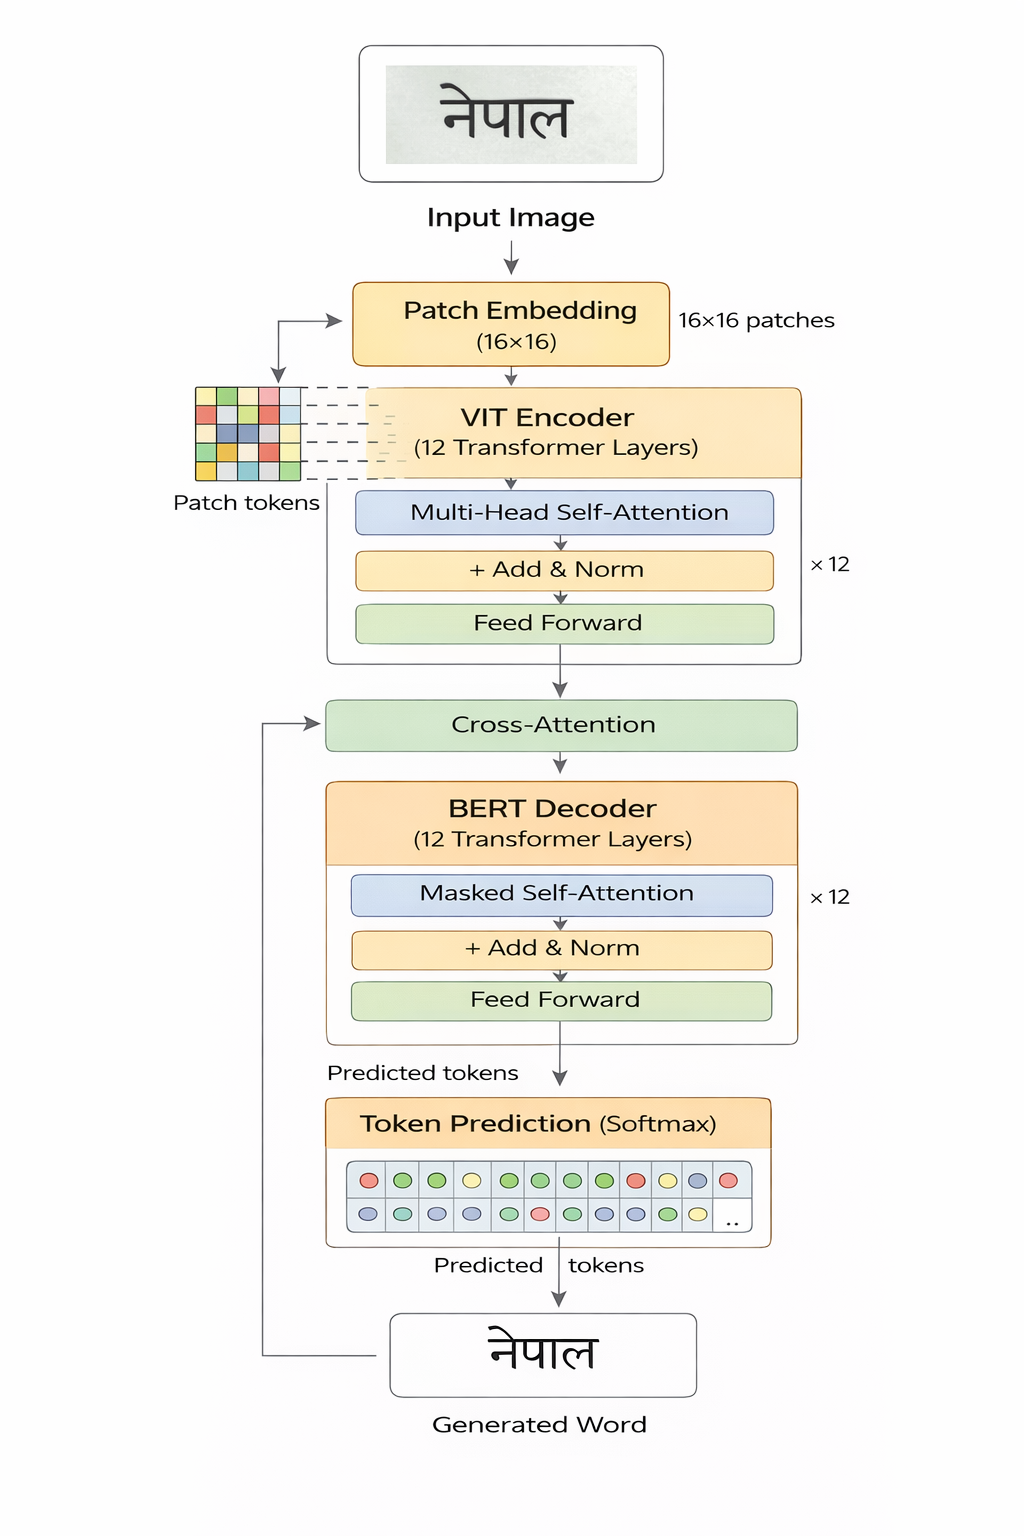
\includegraphics[width=0.80\textwidth]{img/trocr.png}
  \caption{Model Architecture of TrOCR EncoderDecoder Model}
  \label{fig:trocr}
\end{figure}

\subsection{ViT Encoder}

The encoder is a Vision Transformer of the vit-base-patch16-384 variant, with pre-trained weights sourced from microsoft/trocr-base-handwritten;a checkpoint already fine-tuned on handwritten document recognition tasks. This choice provides the model with strong visual priors for cursive and handwritten scripts without requiring training from scratch.

\noindent Each input image is resized to $384 \times 384$ pixels and partitioned
into non-overlapping patches of $16 \times 16$ pixels, yielding 576
patches. Each patch is linearly projected into a 768-dimensional
embedding vector. A learnable \texttt{[CLS]} token is prepended to
the patch sequence, and learnable positional embeddings are added to
each position to preserve spatial structure, resulting in a final
sequence length of 577.

\noindent The sequence is then processed through 12 stacked Transformer blocks.
Each block consists of multi-head self-attention with 12 heads
($d_k = 64$ per head), layer normalisation, residual connections, and
a position-wise feed-forward network with a hidden dimensionality of
3072 and GELU activation. The encoder produces a contextual feature
matrix of shape $[B, 577, 768]$, where $B$ is the batch size. This
output encodes rich spatial and semantic information from the
handwritten word image and serves as the key--value input for the
decoder's cross-attention mechanism.

\subsection{Custom BERT-Based Decoder}

The decoder is a lightweight, custom-built Transformer decoder
constructed using HuggingFace's BertConfig and
BertLMHeadMode. It is intentionally compacted to approximately 4 million parameters for avoiding overfitting on the moderately sized Devanagari training corpus of approximately 70,000 word images.

\noindent The decoder comprises 2 Transformer layers, each with 4 attention
heads and a hidden dimensionality of 256. The feed-forward sub-layer
within each block has an intermediate size of 512 and uses GELU
activation. Dropout with probability 0.1 is applied to both attention
weights and hidden representations for regularisation. The maximum
supported sequence length is 128 token positions.

\noindent At each decoding step, the previously generated token identifiers are
embedded into a 256-dimensional space via a learned token embedding
layer. A causal (left-to-right) masked self-attention mechanism then
allows each position to attend only to prior positions, enforcing
autoregressive generation. Cross-attention is subsequently applied
over the full encoder output, using the encoder's feature matrix as
keys and values and the decoder's current hidden states as queries.
This mechanism enables the decoder to selectively attend to visually
relevant regions of the input image at each character generation step.

\noindent A final linear projection layer maps the decoder's hidden states to
logits over the 112-token vocabulary, from which the most probable
token is selected at each step.

\subsection{Model Integration}

The encoder and decoder are combined into a single trainable model
via VisionEncoderDecoderModel. The decoder start token is
set to \texttt{<s>} (BOS), the padding token to \texttt{<pad>}, and padding positions are masked with $-100$ in the label tensor to exclude them from loss computation. Cross-attention is explicitly enabled in the decoder configuration via the
add\_cross\_attention flag.

Table~\ref{tab:arch} summarises the architectural configuration of
both components.

\begin{table}[H]
\centering
\caption{Model architecture summary}
\label{tab:arch}
\begin{tabular}{lll}
\hline
\textbf{Component} & \textbf{Parameter} & \textbf{Value} \\
\hline
ViT Encoder & Input resolution       & $384 \times 384$ \\
            & Patch size             & $16 \times 16$ \\
            & Sequence length        & 577 (576 patches + CLS) \\
            & Hidden size            & 768 \\
            & Transformer layers     & 12 \\
            & Attention heads        & 12 \\
            & FFN hidden size        & 3072 \\
            & Pre-trained checkpoint & \texttt{trocr-base-handwritten} \\
\hline
BERT Decoder & Transformer layers      & 2 \\
             & Attention heads         & 4 \\
             & Hidden size             & 256 \\
             & FFN intermediate size   & 512 \\
             & Dropout                 & 0.1 \\
             & Max position embeddings & 128 \\
             & Vocabulary size         & 112 \\
             & Initialisation          & Random (from scratch) \\
\hline
\end{tabular}
\end{table}

% ────────────────────────────────────────────────────────────────────
\section{Hyperparameters}

The training configuration was designed to accommodate the two-phase training strategy;an initial decoder-only phase followed by full end-to-end fine-tuning while maintaining training stability through mixed-precision arithmetic, gradient accumulation, and cosine
annealing scheduling.

\subsection{Optimiser}

The AdamW optimiser was used throughout
training, with momentum coefficients $\beta_1 = 0.9$ and
$\beta_2 = 0.999$ and a numerical stability constant of
$\epsilon = 10^{-8}$.

\noindent During Phase~1 (decoder-only training), the encoder parameters were
frozen and only decoder parameters were updated, using a learning rate
of $5 \times 10^{-4}$ with weight decay $10^{-3}$. During Phase~2
(full fine-tuning), differential learning rates were applied:
$5 \times 10^{-7}$ for the encoder, which was already well
pre-trained and required only gentle adaptation, and $5 \times
10^{-5}$ for the decoder. This differential strategy prevents
catastrophic forgetting of the encoder's pre-trained visual
representations while allowing the decoder to continue improving.

\subsection{Learning Rate Scheduler}

A CosineAnnealingWarmRestarts scheduler was applied with a
restart period of $T_0 = 10$ epochs, a restart multiplier of
$T_{\text{mult}} = 1$, and a minimum learning rate of $\eta_{\min} =
10^{-8}$. The periodic warm restarts help the model escape local
minima and explore the loss surface more effectively over longer
training runs.

\subsection{Loss Function}

Label-smoothed cross-entropy loss was used with a smoothing coefficient
of 0.1. Smoothing distributes a small fraction of the probability mass
uniformly across the vocabulary rather than concentrating it entirely
on the ground-truth token, which discourages the model from becoming
overconfident and improves generalisation to unseen character sequences.
Token positions corresponding to padding (label value $= -100$) are
excluded from the loss computation.

\subsection{Training Efficiency}

Mixed-precision training (fp16) was employed via PyTorch's GradScaler to reduce memory consumption and accelerate computation on GPU hardware. Gradient accumulation over 4 steps was
applied, giving an effective batch size of 32 while keeping the per-step memory footprint manageable. Gradient clipping at a maximum norm of 1.0 was applied before each optimiser step to prevent destabilising gradient explosions during early training.

\subsection{Regularisation and Augmentation}

In addition to label smoothing and dropout within the decoder (0.1),
on-the-fly data augmentation was applied exclusively to the training
set to improve robustness to handwriting variation. The augmentation
pipeline comprised Gaussian blur ($p = 0.4$, $\sigma \in [0.1,
1.0]$), random affine transformations (rotation $\pm 7°$, translation
$\pm 7\%$, scale $[0.85, 1.15]$, shear $\pm 5°$), colour jitter
(brightness and contrast $\pm 0.4$, saturation $\pm 0.1$), random
perspective distortion ($p = 0.3$, distortion scale $0.15$), random
autocontrast ($p = 0.2$), and random erasing ($p = 0.3$, erased area
$2\%$--$12\%$ of image area).

\subsection{Early Stopping and Checkpointing}

Validation was performed every 2 epochs on the held-out validation
set. The best model checkpoint was saved whenever a new minimum
validation CER was achieved. Training was terminated early if no
improvement was observed for 10 consecutive validation rounds
(patience $= 10$), corresponding to a maximum of 20 epochs without
progress.

\noindent Table~\ref{tab:hparams} provides a consolidated summary of all
hyperparameter values used during training.

\begin{table}[H]
\centering
\caption{Training hyperparameter summary}
\label{tab:hparams}
\begin{tabular}{lll}
\hline
\textbf{Category} & \textbf{Hyperparameter} & \textbf{Value} \\
\hline
Optimiser & Algorithm            & AdamW \\
          & $\beta_1$, $\beta_2$ & 0.9, 0.999 \\
          & $\epsilon$           & $10^{-8}$ \\
          & Weight decay (Phase 1) & $10^{-3}$ \\
\hline
Learning rate & Phase 1 (decoder only) & $5 \times 10^{-4}$ \\
              & Phase 2 encoder LR     & $5 \times 10^{-7}$ \\
              & Phase 2 decoder LR     & $5 \times 10^{-5}$ \\
\hline
Scheduler & Type                     & CosineAnnealingWarmRestarts \\
          & Restart period $T_0$     & 10 epochs \\
          & Minimum LR $\eta_{\min}$ & $10^{-8}$ \\
\hline
Training & Batch size (per step)      & 8 \\
         & Gradient accumulation      & 4 steps (effective batch 32) \\
         & Gradient clip norm         & 1.0 \\
         & Max epochs                 & 52 \\
         & Validation frequency       & Every 2 epochs \\
         & Early stopping patience    & 10 validation rounds \\
         & Precision                  & fp16 (mixed precision) \\
\hline
Loss & Function        & Cross-entropy \\
     & Label smoothing & 0.1 \\
\hline
Inference & Decoding strategy & Beam search \\
          & Beam width        & 4 \\
\hline
\end{tabular}
\end{table}


\newpage
\section{Performance Evaluation Metrics}

The model was evaluated on the held-out test set of 12,865 word 
images using the following metrics. All string comparisons were 
performed after Unicode NFC normalisation of both predicted and 
ground-truth strings.

\subsection{Character Error Rate (CER)}
CER measures the minimum number of character-level edit operations 
where S,I and D stands for substitutions (S), deletions (D), and insertions (I) required to transform the predicted string into the ground-truth string, 
normalised by the total number of characters $N$ in the ground 
truth. It is computed using the Levenshtein edit distance algorithm. 
A CER of 0 indicates perfect character-level recognition, and it 
served as the primary metric for model selection during training.

\[
\text{CER} = \frac{S + D + I}{N}
\]

\subsection{Word Error Rate (WER)}
WER measures the proportion of test samples for which the predicted 
transcription does not exactly match the ground-truth word label. 
Since each sample in the IIIT-HW-Dev dataset corresponds to a 
single segmented word image, WER directly reflects the rate of 
completely incorrect predictions.

\[
\text{WER} = \frac{\text{Number of incorrectly predicted words}}
                  {\text{Total number of test words}}
\]

\subsection{Exact Match Accuracy}
Exact Match Accuracy measures the proportion of test samples for 
which the model produces a transcription that is identical to the 
ground-truth label in its entirety. It is the complement of WER 
and provides an intuitive measure of end-to-end recognition 
performance.

\[
\text{Exact Match Accuracy} = 
\frac{\text{Number of exactly matched words}}
     {\text{Total number of test words}} \times 100\%
\]

\subsection{Normalised Edit Distance (NED)}
NED provides a length-normalised measure of string similarity 
between the predicted and ground-truth transcriptions. Unlike CER, 
which is normalised by the ground-truth length only, NED normalises 
by the longer of the two strings, making it more robust when 
predicted sequences are significantly shorter or longer than the 
reference. It ranges from 0 (identical strings) to 1 (completely 
dissimilar strings).

\[
\text{NED} = 
\frac{\text{Levenshtein distance}(\hat{y},\, y)}
     {\max\!\left(\lvert\hat{y}\rvert,\,\lvert y\rvert\right)}
\]

\noindent where $\hat{y}$ is the predicted string and $y$ is the 
ground-truth string.


\section{Model Variants Explored}
 
In addition to the NHWDTM system architecture described in Section~3.3, three alternative model configurations were trained on the same dataset and under the same conditions to guide design decisions. The proposed model (v3) was selected as the primary configuration based on its superior downstream performance. Table~\ref{tab:model_variants_ch3} summarises the key
architectural differences across all four variants; quantitative results are reported in \hyperref[chap:Result and Discussion]{Section~5.1}. 


\begin{table}[h!]
\centering
\renewcommand{\arraystretch}{1.8} % Increases row height significantly
\large % <--- This increases the base font size for the table
\resizebox{\textwidth}{!}{%
\begin{tabular}{|p{3cm}|p{4cm}|p{4cm}|p{2.5cm}|p{5cm}|} % Fixed widths allow text to wrap
\hline
\textbf{Model} & \textbf{Encoder} & \textbf{Decoder} & \textbf{Dec. Params} & \textbf{Key Difference} \\ \hline
Baseline & ViT-Base \textit{(trocr-base-handwritten)} & RoBERTa (extended Devanagari vocab) & $\sim$125M & Standard fine-tuning; no custom decoder \\ \hline
TrOCR-Small & ViT-Small \textit{(trocr-small-handwritten)} & Custom BERT (2L / 4H / 256 d) & $\sim$4M & Lighter encoder; faster training \\ \hline
TrOCR-Large & ViT-Large \textit{(trocr-large-handwritten)} & Custom BERT (4L / 8H / 512 d) & $\sim$13M & Maximum encoder capacity \\ \hline
\textbf{Proposed TrOCR base with custom decoder} & \textbf{ViT-Base \textit{(trocr-base-handwritten)}} & \textbf{Custom BERT (2L / 4H / 256 d)} & \textbf{$\sim$4M} & \textbf{Best balance of capacity and efficiency} \\ \hline
\end{tabular}
}
\caption{Model variants explored during development}
\label{tab:model_variants_ch3}
\end{table}